\documentclass{article}
\usepackage{tikz}
\usetikzlibrary{arrows.meta,positioning,calc,shapes.geometric}
\pagestyle{empty}
\begin{document}
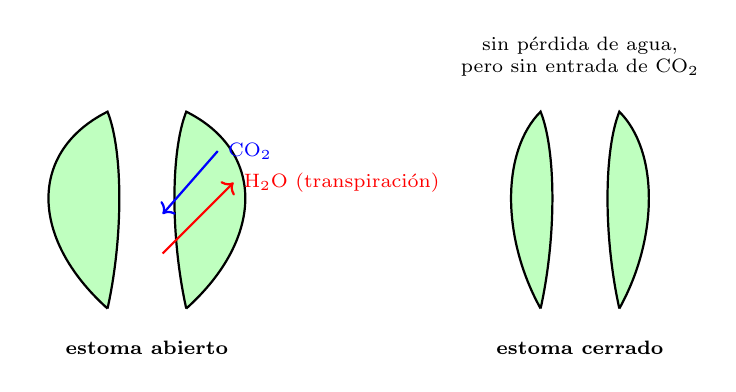
\begin{tikzpicture}
\tikzset{every node/.append style={align=center}}

\foreach \cx/\o/\t in {1.5/0.5/abierto, 7.0/0.0/cerrado} {
  \draw[thick, fill=green!25] (\cx,0) .. controls (\cx-0.5-\o,0.9) and (\cx-0.5-\o,2.0) .. (\cx,2.5) .. controls (\cx+0.2,2.0) and (\cx+0.2,0.9) .. (\cx,0);
  \draw[thick, fill=green!25] (\cx+1.0,0) .. controls (\cx+1.5+\o,0.9) and (\cx+1.5+\o,2.0) .. (\cx+1.0,2.5) .. controls (\cx+0.8,2.0) and (\cx+0.8,0.9) .. (\cx+1.0,0);
  \node[font=\bfseries\scriptsize] at (\cx+0.5,-0.5) {estoma \t};}
\draw[->, thick, blue] (2.9,2.0) -- (2.2,1.2) node[at start, right, font=\scriptsize] {CO$_2$}; \draw[->, thick, red] (2.2,0.7) -- (3.1,1.6) node[at end, right, font=\scriptsize] {H$_2$O (transpiración)};
\node[font=\scriptsize, align=center] at (7.5,3.2) {sin pérdida de agua,\\ pero sin entrada de CO$_2$};

\end{tikzpicture}
\end{document}
